\section{Overlapping Data Transfers}
\label{sec-async}

In this section, we talk about the details of streaming data transfers. Then we go on and talk about how we implement the streaming transfers in Gluon~\cite{dathathri2018gluon}. We then discuss about the implementation and the challenges that we faced during the implementation. 

\subsection{Streaming Data Transfers}

A stream in CUDA is a sequence of operations that execute on the device in the order in which they are issued by the host code. While operations within a stream are guaranteed to execute in the prescribed order, operations in different streams can be interleaved and, when possible, they can even run concurrently. All device operations (kernels and data transfers) in CUDA run in a stream. When no stream is specified, the default stream (also called the “null stream”) is used. The default stream is different from other streams because it is a synchronizing stream with respect to operations on the device: no operation in the default stream will begin until all previously issued operations in any stream on the device have completed, and an operation in the default stream must complete before any other operation (in any stream on the device) will begin.

\begin{figure}
\centering
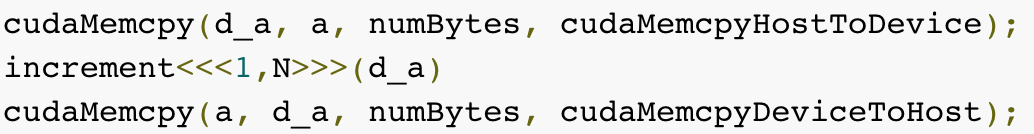
\includegraphics[width=0.49\textwidth]{async-serial.png}
\mycaption{}{This figure shows an algorithm for serially performing communication and computation. }
\label{fig-async-serial}
%\vspace{-20pt}
\end{figure}

\begin{figure}
\centering
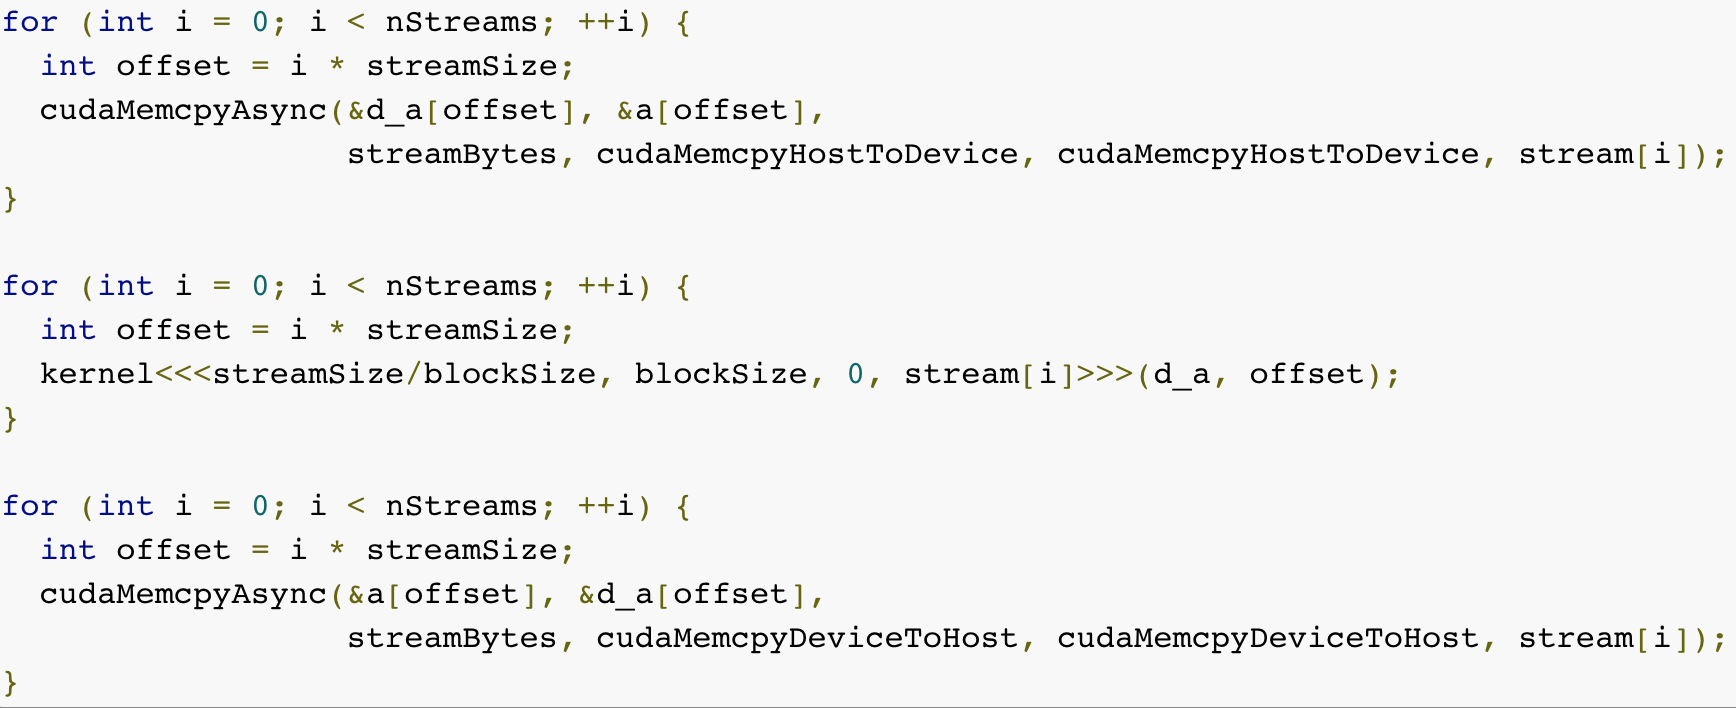
\includegraphics[width=0.49\textwidth]{async-parallel.png}
\mycaption{}{This figure shows an algorithm for overlapping communication and computation. }
\label{fig-async-parallel}
%\vspace{-20pt}
\end{figure}

The main goal behind streaming data transfers is that we want to overlap kernel execution along with data transfers. For this to be successful, the kernel execution and the data transfer should both occur in different, non-default streams. Also, the host memory that is involved in streaming data transfers should be pinned memory, if we want to achieve maximum performance. Figure ~\ref{fig-async-serial} shows the algorithm that uses default stream, which does not overlap computation with communication, whereas Figure~\ref{fig-async-parallel} shows the same algorithm that overlaps computation with communication using non-default streams. Note that both the algorithms provide current results, but the performance varies significantly. 

\begin{figure}
\centering
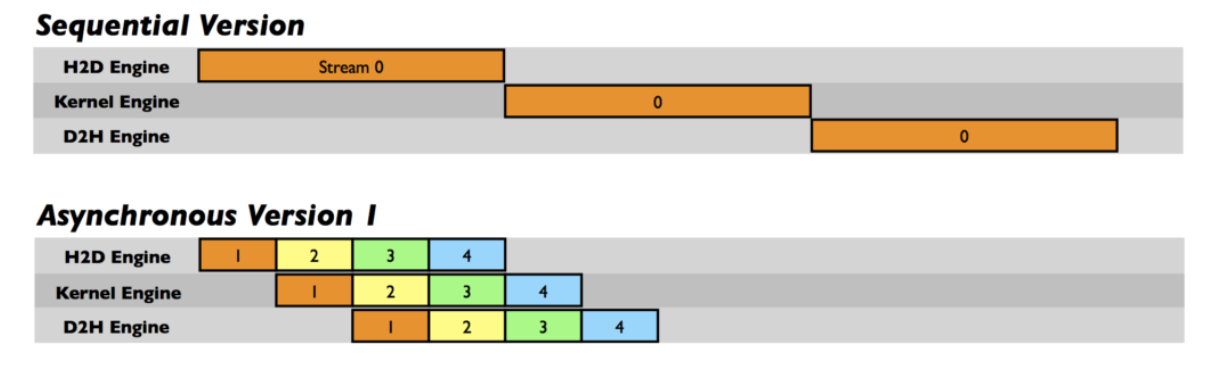
\includegraphics[width=0.49\textwidth]{async-perf.png}
\mycaption{Streaming data performance}{This figure shows the difference in performance between serial and overlapping communication with computation }
\label{fig-async-perf}
%\vspace{-20pt}
\end{figure}

Figure~\ref{fig-async-perf} shows the execution timelines for the sequential algorithm versus the asynchronous algorithm that overlaps computation with communication. As we can see from this figure, the end-to-end latency of the sequential version is roughly 2X compared to the asynchronous version. 

\subsection{Asynchronous Transfers in Gluon}

In the Gluon substrate, during the communication of graph data from a source node (or master node) to a destination node (or mirror node), the following steps take place, in a sequential order:
\begin{enumerate}
\item The offset data of the graph and the bitset data of the graph are computed at the GPU of the source
\item The offset data, bitset data and the shared graph data are copied and serialized into a CPU buffer at the source
\item The CPU buffer is transferred from the source to the destination
\item The CPU buffer at the destination is deserialized and copied to the GPU at the destination
\item The corresponding graph data, offset data and bitset data is computed at the GPU of the destination
\end{enumerate}

We modified these steps that occur during the synchronization phase, and we overlapped the computations in step 1 at the source with the data copy from GPU to CPU in step 2 using asynchronous streaming transfers. At the destination, we overlapped the data copy from CPU to GPU in step 4 with the computation on the copied data in step 5 using asynchronous streaming transfers. 

\subsection{Discussion}

The first challenge that we faced while applying this was to find out exactly where it is possible to apply this optimization in the large code base. We solved this by taking an example of the bfs\_push algorithm that is currently used for communicating the updates of a node in a graph to all its neighbors. Finally we found the point where there were transfers happening between GPU and CPU at the sender and the receiver, and we found opportunity to use this optimization in that part. We believe that it might be possible to apply this optimization to other parts of Gluon too, and this is just our prototype implementation of overlapping data transfers. 

The second challenge was regarding the use of pinned memory for achieving the asynchronous transfers. One limitation of pinned memory is that pinned memory cannot be reallocated or resized once it is allocated. This is an important problem because, in the case of sparse graphs, there is freq	uent resizing of buffers in Gluon, and it is impossible to know the size of the graphs or the number of bits in the bitset and offset to statically determine the size of the buffers. We could not use pinned buffers for this feature, and hence we believe that it won't lead to maximum performance improvements on large graphs. There needs to be a comprehensive change in the code base of Gluon to use pinned memory during the transfers, which might lead to better performance. 




